%
% fig-konform.tex
%
% (c) 2026 Prof Dr Andreas Müller
%
\begin{figure}
\centering
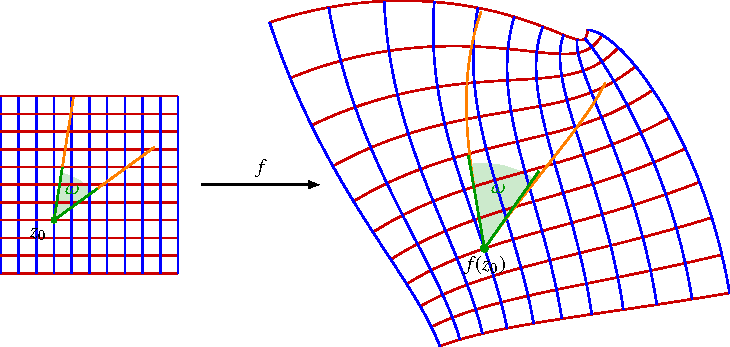
\includegraphics{chapters/020-holomorph/images/konform.pdf}
\caption{Eine holomorph Abbildung $f\colon \mathbb{C}\to\mathbb{C}$
ist konform.
Geraden mit Richtung $w\in\mathbb{C}$, $|w|=1$, durch den Punkt $z_0$
werden auf Kurven ({\color{orange}orange}) durch den Punkt $f(z_0)$
abgebildet, deren Tangenten ({\color{darkgreen}grün}) die Richtung
von $f'(z_0)\cdot w$ haben.
Die Multiplikation mit $f'(z_0)$ ist eine Drehstreckung, die Winkel
erhält.
\label{buch:holomorph:fig:konform}}
\end{figure}
